\chapter{Card Logistics}





\section{Card Types}

There are two primary categories of cards - unit cards (or units for short) and spell cards (or spells for short). Every card has a card `type' associated with it. Spell cards are differentiated in their function and purpose, but are simply a card with the type of `spell'. The unit cards encompass all of the remaining card types. Every unit card also has one or more sub-type(s) (also called secondary type(s)), which is a more focused type specific to the card itself (primarily the art/lore of the unit).

\subsubsection{Types}
The primary types, of which each card is assigned one, are listed below with a brief description.
\begin{description}
	\item[Earth:] Units aligned with nature, resilience, and the physical world. Earth units often have high defense and abilities that enhance survivability.
	\item[Water:] Units embodying fluidity, adaptability, and the power of the seas. Water units typically specialize in control effects and healing.
	\item[Fire:] Units representing destruction, passion, and chaotic power. Fire units are known for high attack values and aggressive effects.
	\item[Air:] Units characterized by speed, agility, and freedom. Air units often have evasion abilities and excel at quick, tactical strikes.
	\item[Electric:] Units aligned with energy, and the power of electricity. Electrical units often have abilities focused on stunning enemies, or interupting other cards.
	\item[Light:] Units symbolizing purity, order, and restoration. Light units frequently provide healing, support, and protective effects.
	\item[Nature:] Units embodying the wild, growth, and the harmony of living things. Nature units often excel in versatility, with abilities that promote regeneration, summon allies, or manipulate the battlefield with natural forces.
	\item[Dark:] Units associated with corruption, death, and forbidden power. Dark units excel at destruction, disruption, and sacrificial effects.
	\item[Spell:] Non-unit cards that represent magical powers, blessings, equipment, spell effects, artifacts, curses, or more. Spells provide a wide range of one-time or ongoing effects to influence the game.
\end{description}

\subsubsection{Sub-Types}
The secondary types, of which each unit card is assigned one or more, are listed below with a brief description.
\begin{description}
	\item[Avian:] Winged creatures of the sky, known for their agility, keen senses, and mastery of aerial maneuvers.
	\item[Dragon:] Powerful, mythical beings with immense strength and destructive capabilities.
	\item[Beast:] Natural creatures with raw physical power, often found in forests and plains.
	\item[Elemental:] Manifestations of elemental forces, bound to the magic of nature.
	\item[Aquatic:] Sea-dwelling creatures adept at controlling water and adapting to fluid environments.
	\item[Warrior:] Skilled fighters trained in physical combat, often acting as frontline attackers.
	\item[Spellcaster:] Mystics and mages who wield magical powers to cast spells and manipulate the battlefield.
	\item[Machine:] Artificial constructs built for labor, warfare, or magical purposes.
	\item[Ghost:] Ethereal spirits bound to the mortal realm, often with abilities to haunt or possess.
	\item[Insect:] Swarming, persistent creatures that thrive in large numbers and rapid reproduction.
	\item[Reptile:] Cold-blooded creatures known for their resilience and venomous strikes.
	\item[Fairy:] Small, magical beings capable of blessings, mischief, and subtle manipulations.
	\item[Undead:] Reanimated corpses and skeletal beings driven by dark magic or lingering souls.
	\item[Botanic:] Living plants and fungal creatures that can entangle foes, spread toxins, or regenerate.
\end{description}




\section{Cards}

\begin{figure}[h]
    \centering
    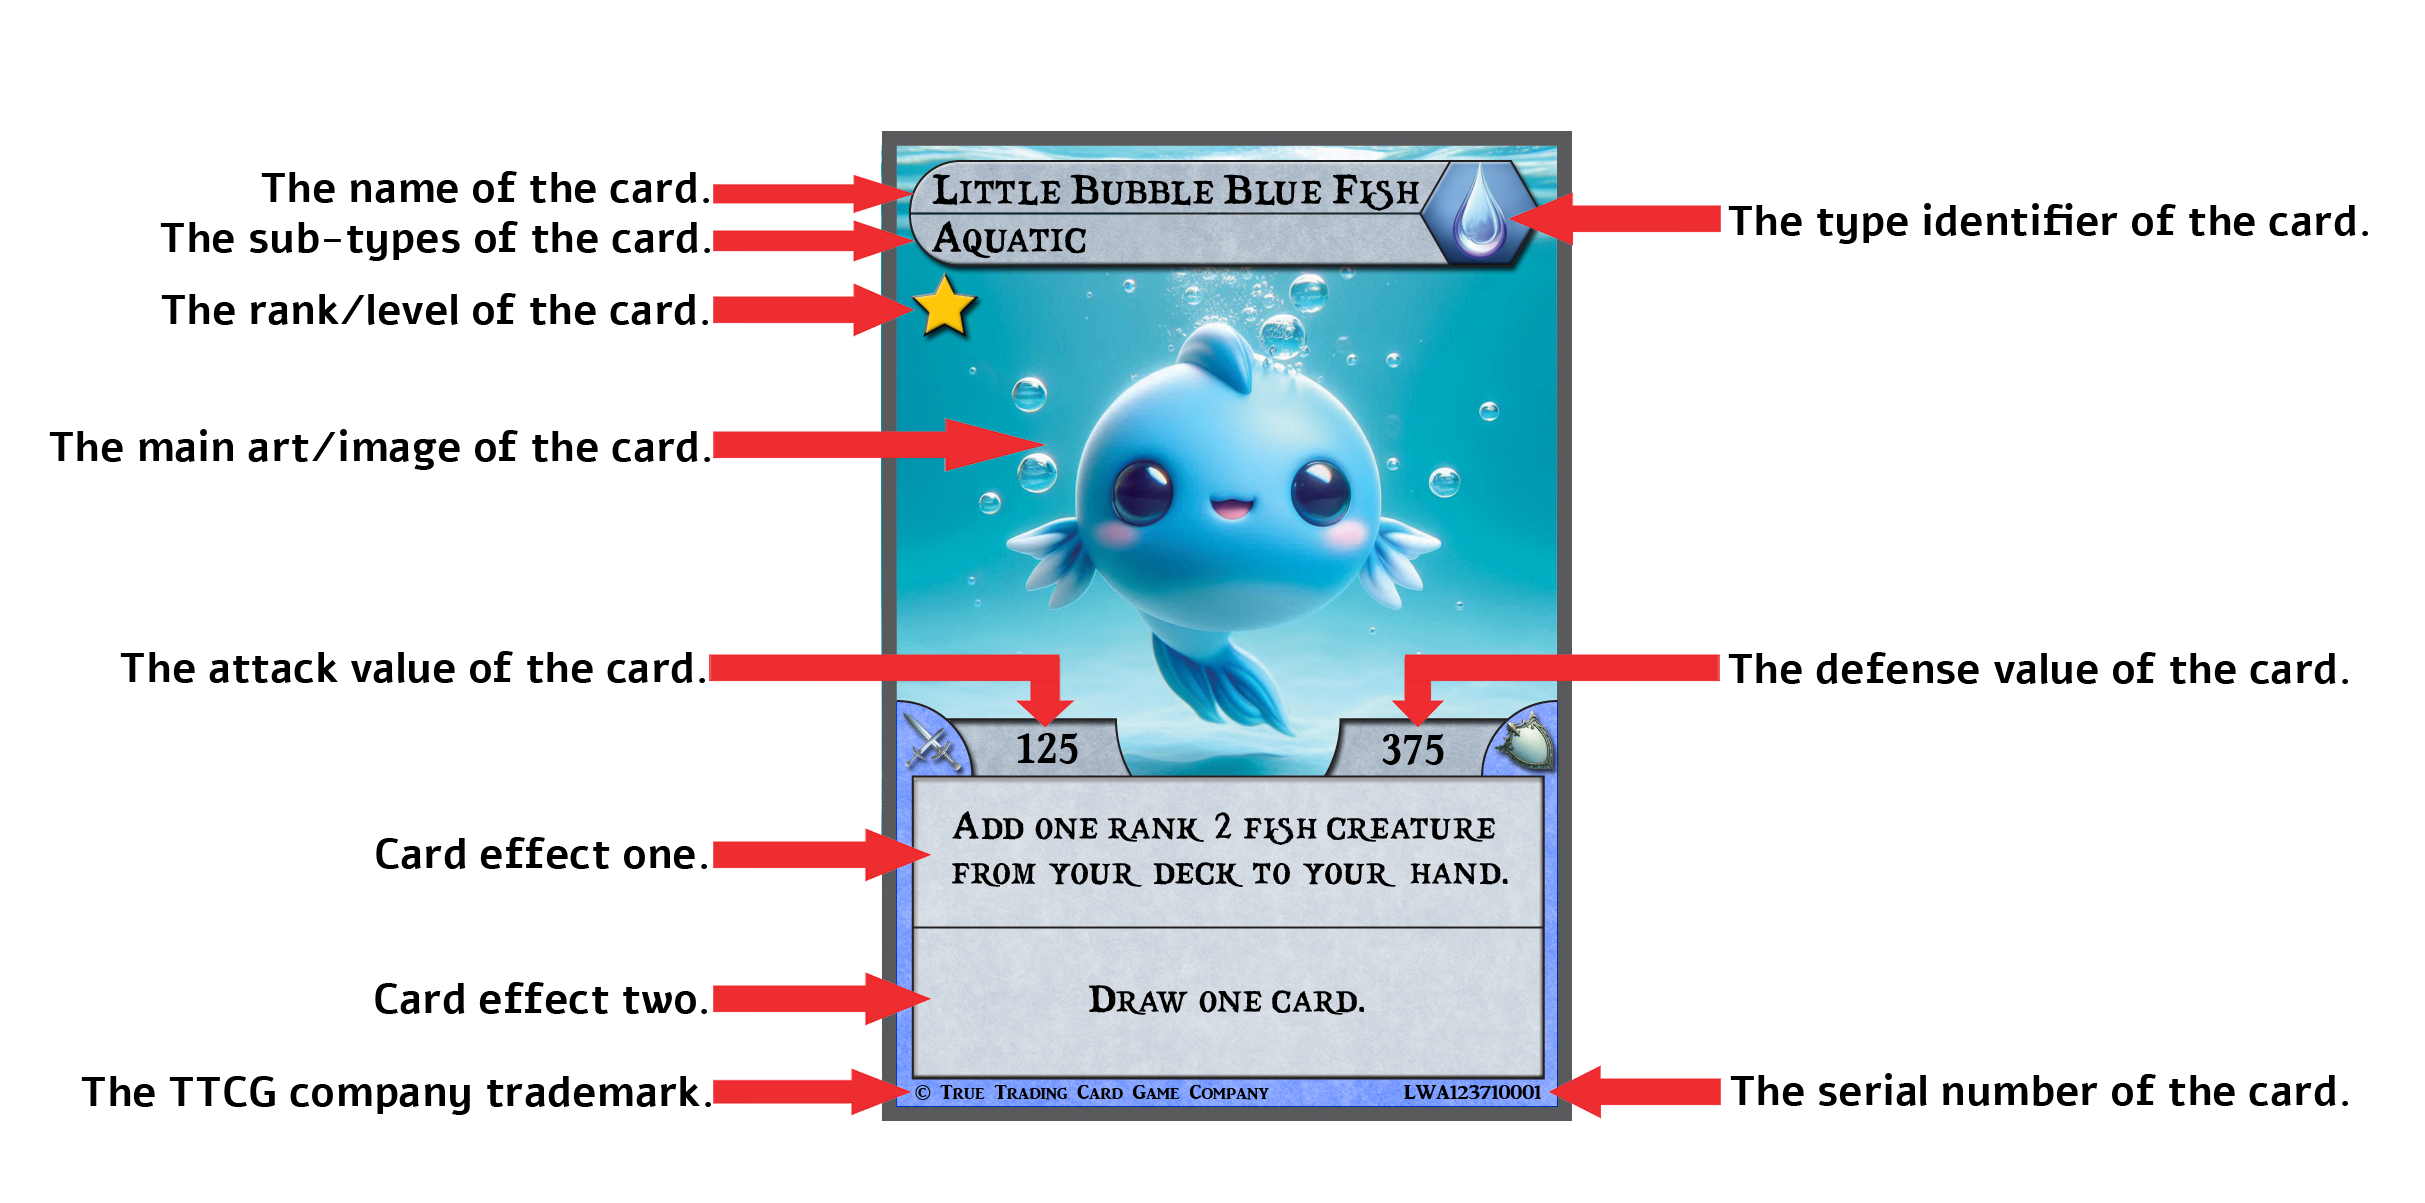
\includegraphics[width=\textwidth]{images/card_details.png} 
    \caption{This is a sample card with a brief explanation for what represents what on the card. This is a rank 1 water unit with a subtype of aquatic.}
    \label{fig:sample_card}
\end{figure}



\subsection{Unit Cards}
// TODO



\subsection{Spell Cards}
// TODO



\subsection{Lore Cards}
// TODO







\section{Effect Variations}
Effects are the core mechanics that drive strategic interaction in the game, modifying the state of play through targeted actions and conditional triggers. Each effect is composed of three key elements: \textit{targets}, which define what the effect applies to; \textit{actions}, which specify what happens to those targets; and \textit{conditions}, which determine when or how the effect can be activated. Targets range from specific cards (e.g., "rank 2 units" or "card(s) under this card") to broad categories (e.g., "all cards" or "opponent’s cards"), allowing for precise or sweeping impacts. Actions encompass a variety of outcomes, such as destroying cards, drawing resources, or modifying stats, shaping the game’s flow and player decisions. Conditions impose requirements or timing, like discarding a card, losing points, or waiting for an attack, adding depth and tactical nuance. Together, these elements create a flexible system where effects can be combined to produce diverse and dynamic gameplay scenarios.

\subsection{Unit Effect Variations}
// TODO

\subsection{Spell Effect Variations}
// TODO


\subsection{Effect Conditions}
Many effects have a condition that must be met in order to use the effect or as part of the effect's actions. A list of these conditions follows with a brief description of what they mean.
\begin{description}
	\item["Discard one card to\dots":] The player must choose and discard one card from their hand to activate the effect of the card. Sometimes this condition is further specific, in which case the player must choose and discard one card matching the exact condition to activate the effect of the card. The  follow-up effect is considered activated after the action of discarding the card.
	\item["Discard this card to\dots":] The player must discard the specific card to trigger its effect, often a one-time cost for a powerful result. The  follow-up effect is considered activated after the action of discarding the card.
	\item["If you have\dots":] A condition based on whether the player has a specific card, type, or number of cards in play or in hand (e.g., "If you have a Fire unit on the field\dots").
	\item["Let your opponent\dots":] The player allows the opponent to perform a specific action or gain some benefit, often with a trade-off for the player. The follow-up effect is considered activated after the action done by the opponent and can only be activated if the opponent successfully takes that action.
	\item["Lose X point(s) to\dots":] The player must sacrifice a certain amount of points (e.g., life points, mana) to trigger the effect. The follow-up effect is considered activated after the player loses the point(s).
	\item["This turn\dots":] The effect lasts or can only be used within the current turn, typically providing a temporary advantage or ability.
	\item["While this card remains on the field\dots":] The effect remains active as long as the card stays in play, often providing continuous benefits or penalties.
	\item["When this card is send to the discard pile\dots":] This effect is triggered when the card is discarded or destroyed, usually offering a secondary benefit upon leaving the field. A card must be considered untapped to activate this effect. The follow-up effect is considered activated after the card is sent to the discard pile.
	\item["When another card is destroyed\dots":] This condition activates the effect when a different card is destroyed, potentially creating a chain reaction. The follow-up effect is considered activated after the other card is destroyed.
	\item["When an enemy card attacks\dots":] The effect activates when an enemy unit declares an attack, providing defensive actions, counterattacks, or interrupts. The follow-up effect is activated before the attack.
	\item["If you control\dots":] A condition based on controlling a specific unit or type of unit, or having a certain number of cards in play.
	\item["At the start of your turn\dots":] The effect triggers automatically at the beginning of the player's turn, typically with a passive or setup ability.
	\item["After this card attacks\dots":] The effect occurs after the card has attacked, often used for follow-up actions or penalties. The follow-up effect is activated after the attack is finished.
	\item["When this card attacks\dots":] The effect occurs after the card has attacked, often used for follow-up actions or penalties. The follow-up effect is activated before the attack.
	\item["During your opponent's phase\dots"]  The effect activates during the opponent's phase (the exact phase will be specified by the card), often to disrupt or delay their strategy.
	\item["When a card effect activates\dots"] The effect activates when another card effect activates. The follow-up effect occurs before the card effect that triggered this card. This is typically known as a counter effect.
	\item["Destroy one card to\dots"] The player must destroy a card they control to activate the effect. The follow-up effect activates after the destruction.
	\item["Destroy this card to\dots"] The player must destroy this card from the field to trigger its effect, often a one-time cost. The follow-up effect activates after destruction.
	\item["Skip your next turn to\dots"] The player must skip their next turn to activate the effect, a significant cost for a powerful outcome. The follow-up effect activates after the turn is skipped.
	\item["Tap\dots", "Untap\dots" ]
\end{description}

    

  
  


\subsection{Effect Targets}
Many effects have targets which the effect applies to. These targets can be broad or specific depending on the effect and all conditions of the target must be met in order for the effect to target that card. These are all pretty precise and straight forward. Regardless, a list of common target formats follows with a brief description of what they mean.
\begin{description}
	\item["one", "two", \dots] Often, an effect specifies a number of cards that its effect applies to. This is straight forward and the number must be adhered to unless another card specifies otherwise.
	\item["rank 1", "rank 2", \dots] Often, a specific rank of card is specified in the target. This must be a card matching that rank value.
	\item["rank x or lower"] This represents a card matching the rank or having a rank lower than the rank specified. 
	\item["rank x or higher"]  This represents a card matching the rank or having a rank higher than the rank specified. 
	\item["dark", "light", "spell", \dots] Often, a card will specify a type of card in the target. This type must be adhered to.
	\item["dragon", "warrior", \dots] Often, a card will specify a sub-type of card in the target. This type must be adhered to.
	\item["this card"] The effect targets the card it is currently associated with, often used for self-targeting abilities.
	\item["all cards", "each"] A broad target that includes all cards of a specified type or set. For example, "all Fire-type units" or "each unit on the field."
	\item["opponent's cards"] Specifies that the target is the opponent's cards, often used for disrupting or removing enemy units or spells.
	\item["your cards"] Specifies that the target is your own cards, often for protection or support abilities that affect your side of the field.
	\item["lowest attack", "highest defense", \dots] A conditional target based on the card’s stats. For example, "lowest attack" targets the card with the lowest attack value.
	\item["in your hand", "in your discard pile", "in your deck", \dots] Specifies cards in specific locations, such as those in the player's hand or discard pile.
	\item["equipped unit"] Targets a unit that is currently equipped with an item or equipment card.
	\item["another card on the field."] This would be any card on either player's side of the field. There must be another card on the field other than the card that says this to activate this effect.
	\item["another card on your side of the field."] This would be any card on your side of the field. There must be another card on the field other than the card that says this to activate this effect.
	\item["card(s) under this card"] This is a card that is physically underneath the card in question (not to be confused with \textit{below} the card on the field).
	\item["card(s) under another card"] Targets any card(s) physically underneath a different card on the field, distinct from the card with the effect.
	\item["card(s) below this card"] This is a card that is \textit{below} the card in questions position on the field - such as a spell card below a unit (not to be confused with \textit{under} a card).
\end{description}
The targets of a card can be any combination of the above descriptors or other possible card features.



\subsection{Effect Actions}
Effect actions define what an effect does to the targeted cards or entities. These actions are typically used in the effect’s resolution and determine how the game state is modified. Below is a list of common effect actions with a brief description of each:

\begin{description}
	\item[Destroy] The target card is removed from the field and sent to the discard pile. This action usually eliminates the target from play completely.  
	\item[Send] The target card is moved from one place to another, such as from the field to the discard pile, from hand to deck, or other designated zones depending on the effect.  
	\item[Mill] The target card or cards are placed from the top of a deck into the discard pile, often used to deplete the opponent's deck or trigger discard-related effects.  
	\item[Discard] The target card is taken from the player's hand and placed in the discard pile, typically reducing resources or disrupting the opponent’s strategy.  
	\item[Counter] The target card’s effect is negated or stopped entirely. A counter might prevent the resolution of a spell, effect, or action from the opponent, nullifying its effect.
	\item[Return] The target card is returned to its previous location or zone, such as returning a card from the field to the hand, deck, or another appropriate zone.  
	\item[Equip] A specific piece of equipment is attached to a target card, usually a unit, granting it additional abilities or buffs.  
	\item[Activate] The effect triggers or activates a specified ability or action on a card, often requiring specific conditions or costs to be met.  
	\item[Add] The effect adds a specified card or value to a target card, player, or zone. For example, adding cards to a player’s hand.  
	\item[Shuffle] The target cards are shuffled back into the deck, discard pile, or any other designated zone. This is often used to obscure the order of cards and introduce randomness.  
	\item[Reveal] The target card is revealed face-up to all players, usually as a means of providing information or triggering specific effects based on visibility.  
	\item[Search] The player may search through their deck, hand, for a specific card, typically allowing for strategic card retrieval.  
	\item[Gain] The target card or player gains a benefit, such as life points, attack points, defense points, or other advantages.  
	\item[Lose] The target card or player loses a specified amount of points, attack, defense, or other metric.  
	\item[Skip] The target player or card’s action is skipped, preventing them from performing a certain action, such as skipping a phase or a turn.
	\item[Draw] Moves cards from the top of the deck to the hand, increasing available resources.
	\item[Play] Places a card into active use on the field from a zone (e.g., hand, discard pile).
	\item[Place] Positions a card in a specific location (e.g., under another card).
	\item[Swap] Exchanges the position of two cards or swaps their stats (e.g., Attack and Defense).
	\item[Prevent] Stops a specified action from activating or affecting a target (e.g., preventing destruction).
	\item[Modify] Alters a card’s stats, rank, or type (e.g., increasing rank or doubling Attack).
	\item[Rank Up] Stacking a card of one higher rank on top of a card.
\end{description}






















